\documentclass[12pt]{ctexart}
\usepackage{geometry}       % 设置页面整体布局
\geometry{top=2.5cm, bottom=2.5cm, left=2cm, right=2cm}
\usepackage{fancyhdr}       % 设置页眉页脚布局
\pagestyle{fancy}
\rhead{\thepage}            % 设置右页眉为页数
\chead{中国科学技术大学}
\cfoot{}                    % 设置中间页脚为空
\usepackage{amsmath}        % 数学公式宏包
\numberwithin{equation}{section}
\usepackage{esint}          % 交叉引用宏包
\usepackage[colorlinks,     % 设置引用的颜色
            linkcolor=black,
            anchorcolor=black,
            urlcolor=cyan,
            citecolor=black,
           ]{hyperref}
\usepackage{makecell}       % 插入表格宏包
\usepackage{longtable}      % 长表格宏包
\usepackage{appendix}       % 生成附录宏包
\usepackage{graphicx}       % 插入图片宏包
\usepackage{epstopdf}       % 插入eps图片宏包
\usepackage{cite}           % 文献引用宏包
\renewcommand{\thefigure}   % 设置图片编号格式
    {\thesection{}.\arabic{figure}}
\renewcommand{\thefootnote}{} % 设置角标编号不出现在文中
                            % 以\footnotetext{Footnotetext without footnote mark}使用
\usepackage{unicode-math}
\usepackage{listings}
\usepackage{hyperref}



\CTEXsetup[format={\Large\bfseries}]{section}

\begin{document}

\nocite{*}

\begin{center}
    \heiti \fontsize{24pt}{0}{燃烧热的测定}

    \vspace{12pt}

    \kaishu \fontsize{13.75pt}{0}禤科材
    

    \footnotetext{\textbf{实验日期:}2022年12月9日}
    \footnotetext{\textbf{作者简介:}禤科材(2002-),男,学号PB20030874,中国科学技术大学本科在读,专业方向为化学物理}
    \footnotetext{\textbf{联系方式:}电话 18108064415 ,邮箱 \href{mailto:ustcxkc@mail.ustc.edu.cn}{ustcxkc@mail.ustc.edu.cn}}

    \vspace{5pt}

    \songti \fontsize{12pt}{0}(中国科学技术大学化学与材料科学学院,安徽 合肥 230026)
\end{center}

\noindent\textbf{摘~~~\!要}~~~\!
有机物完全燃烧时,会放出大量热量。本次实验用氧弹测定萘的燃烧热。
氧弹具有操作方便,结果准确等优点。在恒容容器中通入氧气使萘完全燃烧,
用热容已知的介质将热量完全吸收,通过测量该介质的温度变化即可得出
较为准确的燃烧热数值。同时,实验还通过雷诺图校正减小了环境热交换
对结果的影响。
\newline
\textbf{关键字}~~~\!
氧弹量热法、苯甲酸、萘

\begin{center}
    {\LARGE\rmfamily\textbf{Determination of Combustion Heat of Naphthalene by Oxygen Bomb Calorimeter}}

    \vspace{12pt}

    {\slshape Xuan Kecai}

    \vspace{5pt}

    (School of Chemistry and Material Science, USTC, Hefei 230026, China)
\end{center}

\noindent\textbf{Abstract}~~~\!
When organic matter is completely burned, it will release
a lot of heat. In this experiment, the combustion heat of
naphthalene was measured by oxygen bomb. The oxygen bomb has
the advantages of convenient operation and accurate results.
Oxygen is introduced into the constant volume container to
completely burn naphthalene, and the heat is completely
absorbed by a medium with known heat capacity. A more
accurate combustion heat value can be obtained by measuring
the temperature change of the medium. At the same time,
the influence of environmental heat exchange on the results
is reduced by renogram correction.
\newline
\textbf{Keywords}~~~\!
Oxygen bomb calorimetry; benzoic acid; naphthalene

\section{序言}

热力学中,反应热一直是一个重要却难以测量的物理量。由已知反应的热效应,
通过Hess定律可以计算出许多难以测定反应热的反应的热效应。燃烧热是
反应热的一种,通过弹式量热计我们可以较为方便的测量燃烧热。$^{[1]}$
由热力学第一定律,恒容热效应$Q_V$与恒压热效应$Q_P$有如下关系$^{[2]}$
\begin{align}
    Q_P = Q_V + \Delta nRT
\end{align}
其中$\Delta n$为反应前后气态物质的物质的量之差,$R$为气体摩尔常数,
$T$为反应环境的开尔文温度。

本实验中使用恒温氧弹量热计测量等容燃烧热,燃烧的引线为Cu-Ni合金丝,
恒温氧弹量热计的热容为
\begin{align}
    C_{\text{装置}} = \frac{Q}{\Delta T}
    = \frac{mQ_V - 3242 m_{\text{消耗的金属丝}}}{\Delta T}
\end{align}
通过用标准物质苯甲酸对装置热熔进行标定,我们可以算出目标燃烧物的燃烧热。

\section{实验}
\subsection{试剂与仪器}
苯甲酸(AR,国药集团化学试剂有限公司),萘(AR,国药集团化学试剂有限公司)等。

HR-15B型氧弹式量热计(南京南大万和科技有限公司)、NTY-10A型数字式
千分温度计(南京南大万和科技有限公司)、BH-IIS型燃烧热数据采集接口装置
(南京南大万和科技有限公司)、SQP型电子分析天平(Sartorius)、
769YP-15A粉末压片机(天津市科器高新技术公司)、MF500B型万用表
(上海第四电表厂有限公司)、移液管、洗耳球等。

\subsection{实验方法}
\subsubsection{测量实验体系的热容}
(1)样品压片:用分析天平称量约0.8g苯甲酸。用直尺量取一根长度约为20cm的
细Cu-Ni合金丝,并准确称量其质量。将金属丝与苯甲酸放入模具中,在
0.8$\sim$1MPa下压片。将压片固定在氧弹内。

(2)搭建装置和测量:向氧弹中充入高压氧气,在水槽中加入3000.00mL水,
放入氧弹式量热计,调节温度使内层温度比外层温度低0.78$\sim$0.80$^\circ$C,
点火,测量水温变化。

(3)称量检查:取出氧弹并放气,观察苯甲酸是否燃烧尽,称量剩余合金丝的质量。

\subsubsection{测量萘的燃烧热}
重复2.2.1节的实验步骤,将0.8g苯甲酸换为0.6g萘,将压片压力换为0.5MPa。

\section{结果与讨论}
\subsection{实验结果}
图3.1和图3.2分别为苯甲酸和萘燃烧时体系的温度变化曲线。
\begin{figure}[!h]
\begin{minipage}[t]{0.5\linewidth}
    \centering
    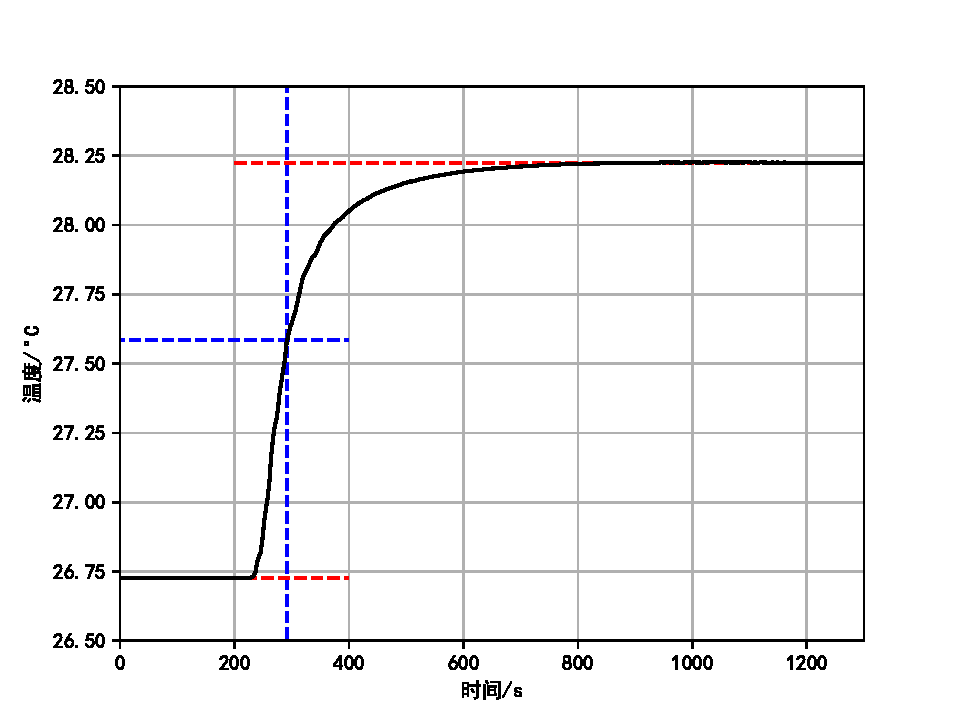
\includegraphics[scale=0.6]{ben.pdf}
    \caption{苯甲酸燃烧的温度-时间曲线}
\end{minipage}
\begin{minipage}[t]{0.5\linewidth}
    \centering
    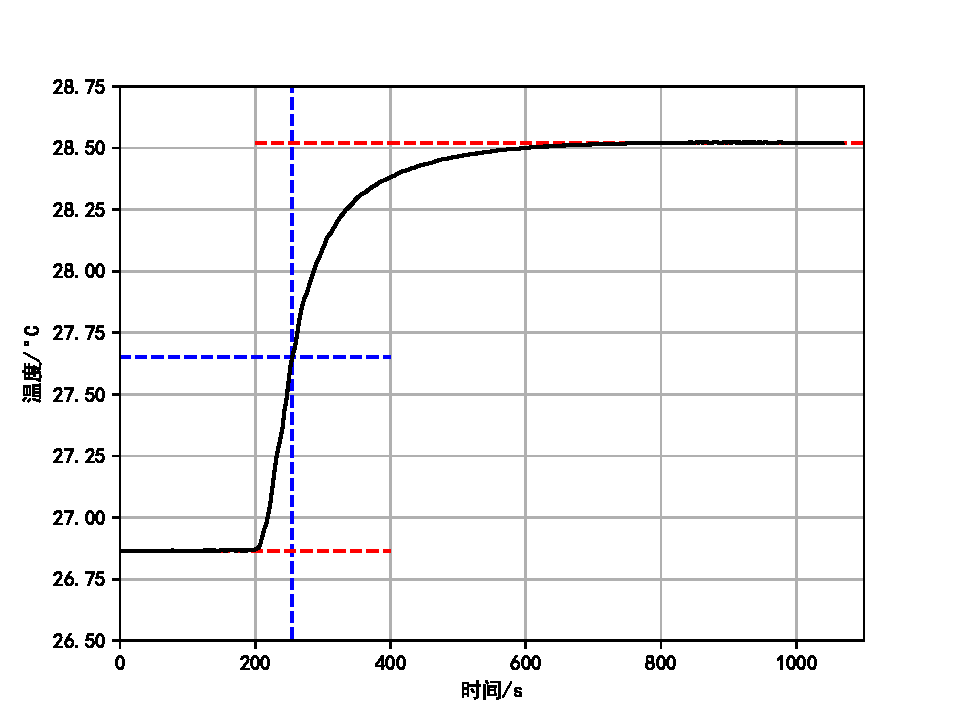
\includegraphics[scale=0.6]{nai.pdf}
    \caption{萘燃烧的温度-时间曲线}
\end{minipage}
\end{figure}

经计算可得反应体系的热熔为$C = -1.457\times 10^4$J/K,萘的
等容热效应为$Q_V = -5185.58$kJ/mol,等压热效应为
$Q_P = -5190.58$kJ/mol。故萘的燃烧热为$5190.58$kJ/mol,
与理论值$5153.9$kJ/mol相比,相对误差为$0.71\%$。

\subsection{误差分析}
\subsubsection{系统误差}
(1)萘易升华,实际燃烧质量会偏少。

(2)温度计等仪器有精度误差。

(3)实验仪器无法做到完全绝热,导致实验结果与理论值有偏差。

(4)实际气体仅近似满足理想气体状态方程,会与理论结果有偏差。

(5)压片由固态燃烧变为二氧化碳气体和液态水,有体积改变。

\subsubsection{偶然误差}
(1)固定压片时会有细小粉末从压片上脱落,造成实际燃烧质量偏少。

(2)合金丝融化为小球状并黏附在金属杆上,难以完整取出,质量测量不够准确。

\subsection{实验拓展}
任冬梅等人$^{[3]}$针对实验中存在的点火成功率较低的问题,从引线材质,
待测物质的理化性质等方面进行分析与改进,将实验成功率提高了$23\%$,
实验的平均相对标准偏差为$3.2\%$,提高了实验效率与结果精度。

\section{结语}
本实验通过氧弹量热计测定萘的燃烧热,通过实验测得反应体系的热容为
$C = -1.457\times 10^4$J/K,萘的等容热效应为$Q_V = -5185.58$
kJ/mol,等压热效应为$Q_P = -5190.58$kJ/mol。因此,萘的燃烧热为
$5190.58$kJ/mol,与理论值$5153.9$kJ/mol的相对误差为$0.71\%$。
实验操作较为容易,但要注意固定金属丝以保证点火成功。此外,还搜索了
可行的改进方案,使实验测定结果更为准确。

\begin{center}
    \Large\bfseries{参考文献}
\end{center}
\noindent
[1] 傅献彩, 沈文霞, 姚天扬等. 物理化学(第五版). 上册[M]. 高等教育出版社,2006.

\noindent
[2] 张祖德. 无机化学. 修订版[M]. 中国科学技术大学出版社, 2010.

\noindent
[3] 任冬梅, 高鸽, 刘鑫, 赵岩, 夏云生, 包德才. “燃烧热测定”实验的改进[J]. 科技创新与应用, 2017,35(25).

\newpage

\begin{center}
    \LARGE\bfseries{附件~~~实验数据处理}
\end{center}
\begin{center}
    \Large\bfseries{附件I~~~实验记录原始数据}
\end{center}

\subsubsection*{苯甲酸燃烧热的测定数据}
苯甲酸质量:0.8288g

金属丝质量:0.0128g

压片质量:0.8412g

残余金属丝质量:0.0011g

反应前外套温度:27.545$^\circ$C

反应后外套温度:27.623$^\circ$C

\subsubsection*{萘燃烧热的测定数据}

萘质量:0.6083g

金属丝质量:0.0143g

压片质量:0.6198g

残余金属丝质量:0.0042g

反应前外套温度:27.627$^\circ$C

反应后外套温度:27.680$^\circ$C

\begin{center}
    \Large\bfseries{附件II~~~实验数据处理}
\end{center}
\subsection*{II.1~~~温度的校正}
如图3.1和3.2所示是两种物质燃烧时外层温度随时间变化的曲线,取反应
前后的温度分别做线性拟合,可以得到温度的校正值。

\subsubsection*{苯甲酸温度的校正}
外界温度为
\begin{align*}
    T = \frac{27.545 + 27.623}{2} = 27.584~(^\circ\mathrm{C})
\end{align*}
该温度对应的时间为292s。分别取0$\sim$225s和930$\sim$1300s的数据
进行线性拟合,得到
\begin{align*}
    y &= 0.000x + 26.727 \\
    y &= 0.000x + 28.234
\end{align*}
拟合的直线几乎水平。代入$x = $292s,得到对应的温度值分别为
26.727$^\circ$C和28.234$^\circ$C。温差为$\Delta T = 1.507^\circ$C。

\subsubsection*{萘温度的校正}
外界温度为
\begin{align*}
    T = \frac{27.627 + 27.680}{2} = 27.654~(^\circ\mathrm{C})
\end{align*}
该温度对应的时间为254.5s。分别取0$\sim$180s和850$\sim$1000s的数据
进行线性拟合,得到
\begin{align*}
    y &= 0.000x + 26.864 \\
    y &= 0.000x + 28.525
\end{align*}
拟合的直线几乎水平。代入$x = $292s,得到对应的温度值分别为
26.864$^\circ$C和28.525$^\circ$C。温差为$\Delta T = 1.679^\circ$C。

\subsection*{II.2~~~燃烧热的计算}
用苯甲酸燃烧的等容热效应标定出装置的热容为
\begin{align*}
    C_{\text{装置}} &= \frac{mQ_V - 3242m_{\text{消耗的金属丝}}}{\Delta T} \\
    &= \frac{(0.8412 - 0.0128)\times (-26460) - 3242\times (0.0128 - 0.0011)}{1.507} \\
    &= -1.457\times 10^4~(\mathrm{J/K})
\end{align*}
萘的摩尔质量为128.18g/mol,故萘的燃烧热的等容热效应为
\begin{align*}
    Q_V &= \frac{C{\text{装置}\Delta T + 3242m_{\text{消耗的金属丝}}}}{m}\times M \\
    &= \frac{-1.457\times 10^4\times 1.679 + 3242\times(0.0143-0.0042)}{0.6198 - 0.0143} \times 128.18\times 10^{-3} \\
    &= -5185.58~(\mathrm{kJ/mol})
\end{align*}
由萘燃烧的化学反应方程式
\begin{align*}
    \mathrm{C_{10}H_8(s) + 12O_2(g) \rightarrow 10CO_2(g) + 4H_2O(l)}
\end{align*}
得$\Delta n = -2$,故萘燃烧的等压热效应为
\begin{align*}
    Q_P &= Q_V + \Delta nRT \\
    &= -5185.58 + (-2)\times 8.314 \times 10^{-3} \times (273.15 + 27.654) \\
    &= -5190.58~\mathrm{(kJ/mol)}
\end{align*}
因此萘的燃烧热为5190.58kJ/mol。萘的理论燃烧热为5153.9kJ/mol,
故相对误差为0.71\%。

\begin{center}
    \Large\bfseries{附件III~~~燃烧热仪器记录数据}
\end{center}

\begin{longtable}{cc|cc|cc|cc|cc}
    \caption{苯甲酸燃烧温度-时间原始数据} \\
    % 设置表头
    \hline
    t(s) & T($^\circ$C) & t(s) & T($^\circ$C) & t(s) & T($^\circ$C) & t(s) & T($^\circ$C) & t(s) & T($^\circ$C) \\
    \hline
    \endhead
    % 设置表尾
    \hline
    \endfoot
    3        & 26.727   & 6        & 26.727   & 9        & 26.727   & 12       & 26.727   & 15       & 26.727   \\
    18       & 26.727   & 21       & 26.727   & 24       & 26.727   & 27       & 26.727   & 30       & 26.727   \\
    33       & 26.727   & 36       & 26.727   & 39       & 26.726   & 42       & 26.727   & 45       & 26.727   \\
    48       & 26.727   & 51       & 26.727   & 54       & 26.727   & 57       & 26.727   & 60       & 26.727   \\
    63       & 26.727   & 66       & 26.727   & 69       & 26.726   & 72       & 26.726   & 75       & 26.727   \\
    78       & 26.727   & 81       & 26.726   & 84       & 26.727   & 87       & 26.726   & 90       & 26.726   \\
    93       & 26.726   & 96       & 26.727   & 99       & 26.727   & 102      & 26.727   & 105      & 26.727   \\
    108      & 26.726   & 111      & 26.727   & 114      & 26.726   & 117      & 26.726   & 120      & 26.727   \\
    123      & 26.726   & 126      & 26.727   & 129      & 26.727   & 132      & 26.726   & 135      & 26.726   \\
    138      & 26.727   & 141      & 26.726   & 144      & 26.727   & 147      & 26.727   & 150      & 26.727   \\
    153      & 26.727   & 156      & 26.727   & 159      & 26.727   & 162      & 26.727   & 165      & 26.727   \\
    168      & 26.727   & 171      & 26.726   & 174      & 26.727   & 177      & 26.727   & 180      & 26.727   \\
    183      & 26.727   & 186      & 26.727   & 189      & 26.727   & 192      & 26.727   & 195      & 26.727   \\
    198      & 26.727   & 201      & 26.727   & 204      & 26.727   & 207      & 26.727   & 210      & 26.728   \\
    213      & 26.727   & 216      & 26.727   & 219      & 26.727   & 222      & 26.727   & 225      & 26.727   \\
    228      & 26.728   & 231      & 26.730   & 234      & 26.735   & 237      & 26.750   & 240      & 26.788   \\
    243      & 26.805   & 246      & 26.821   & 249      & 26.869   & 252      & 26.931   & 255      & 26.976   \\
    258      & 27.014   & 261      & 27.073   & 264      & 27.162   & 267      & 27.223   & 270      & 27.270   \\
    273      & 27.295   & 276      & 27.338   & 279      & 27.395   & 282      & 27.436   & 285      & 27.478   \\
    288      & 27.515   & 291      & 27.574   & 294      & 27.603   & 297      & 27.630   & 300      & 27.645   \\
    303      & 27.667   & 306      & 27.684   & 309      & 27.713   & 312      & 27.744   & 315      & 27.772   \\
    318      & 27.797   & 321      & 27.820   & 324      & 27.830   & 327      & 27.844   & 330      & 27.855   \\
    333      & 27.872   & 336      & 27.885   & 339      & 27.888   & 342      & 27.896   & 345      & 27.909   \\
    348      & 27.927   & 351      & 27.940   & 354      & 27.951   & 357      & 27.962   & 360      & 27.968   \\
    363      & 27.974   & 366      & 27.979   & 369      & 27.987   & 372      & 27.995   & 375      & 28.006   \\
    378      & 28.010   & 381      & 28.016   & 384      & 28.020   & 387      & 28.025   & 390      & 28.030   \\
    393      & 28.037   & 396      & 28.045   & 399      & 28.048   & 402      & 28.054   & 405      & 28.059   \\
    408      & 28.065   & 411      & 28.069   & 414      & 28.074   & 417      & 28.078   & 420      & 28.081   \\
    423      & 28.086   & 426      & 28.090   & 429      & 28.092   & 432      & 28.095   & 435      & 28.099   \\
    438      & 28.103   & 441      & 28.107   & 444      & 28.111   & 447      & 28.114   & 450      & 28.115   \\
    453      & 28.117   & 456      & 28.120   & 459      & 28.123   & 462      & 28.125   & 465      & 28.128   \\
    468      & 28.130   & 471      & 28.132   & 474      & 28.134   & 477      & 28.136   & 480      & 28.139   \\
    483      & 28.141   & 486      & 28.143   & 489      & 28.145   & 492      & 28.147   & 495      & 28.150   \\
    498      & 28.152   & 501      & 28.153   & 504      & 28.154   & 507      & 28.157   & 510      & 28.157   \\
    513      & 28.159   & 516      & 28.160   & 519      & 28.162   & 522      & 28.164   & 525      & 28.165   \\
    528      & 28.166   & 531      & 28.168   & 534      & 28.169   & 537      & 28.170   & 540      & 28.172   \\
    543      & 28.174   & 546      & 28.174   & 549      & 28.176   & 552      & 28.177   & 555      & 28.178   \\
    558      & 28.179   & 561      & 28.179   & 564      & 28.181   & 567      & 28.182   & 570      & 28.183   \\
    573      & 28.184   & 576      & 28.184   & 579      & 28.186   & 582      & 28.187   & 585      & 28.188   \\
    588      & 28.189   & 591      & 28.190   & 594      & 28.190   & 597      & 28.190   & 600      & 28.192   \\
    603      & 28.194   & 606      & 28.194   & 609      & 28.195   & 612      & 28.195   & 615      & 28.196   \\
    618      & 28.197   & 621      & 28.197   & 624      & 28.198   & 627      & 28.198   & 630      & 28.200   \\
    633      & 28.200   & 636      & 28.201   & 639      & 28.201   & 642      & 28.202   & 645      & 28.203   \\
    648      & 28.203   & 651      & 28.204   & 654      & 28.204   & 657      & 28.205   & 660      & 28.206   \\
    663      & 28.205   & 666      & 28.207   & 669      & 28.207   & 672      & 28.207   & 675      & 28.207   \\
    678      & 28.208   & 681      & 28.208   & 684      & 28.209   & 687      & 28.209   & 690      & 28.210   \\
    693      & 28.210   & 696      & 28.210   & 699      & 28.211   & 702      & 28.211   & 705      & 28.212   \\
    708      & 28.212   & 711      & 28.212   & 714      & 28.213   & 717      & 28.213   & 720      & 28.213   \\
    723      & 28.214   & 726      & 28.214   & 729      & 28.214   & 732      & 28.215   & 735      & 28.215   \\
    738      & 28.216   & 741      & 28.216   & 744      & 28.215   & 747      & 28.216   & 750      & 28.216   \\
    753      & 28.217   & 756      & 28.217   & 759      & 28.217   & 762      & 28.217   & 765      & 28.218   \\
    768      & 28.218   & 771      & 28.219   & 774      & 28.219   & 777      & 28.219   & 780      & 28.219   \\
    783      & 28.220   & 786      & 28.219   & 789      & 28.220   & 792      & 28.220   & 795      & 28.220   \\
    798      & 28.220   & 801      & 28.220   & 804      & 28.220   & 807      & 28.220   & 810      & 28.221   \\
    813      & 28.221   & 816      & 28.221   & 819      & 28.221   & 822      & 28.221   & 825      & 28.221   \\
    828      & 28.222   & 831      & 28.222   & 834      & 28.222   & 837      & 28.222   & 840      & 28.223   \\
    843      & 28.223   & 846      & 28.223   & 849      & 28.223   & 852      & 28.223   & 855      & 28.223   \\
    858      & 28.224   & 861      & 28.224   & 864      & 28.223   & 867      & 28.224   & 870      & 28.224   \\
    873      & 28.224   & 876      & 28.224   & 879      & 28.224   & 882      & 28.224   & 885      & 28.224   \\
    888      & 28.224   & 891      & 28.224   & 894      & 28.225   & 897      & 28.225   & 900      & 28.224   \\
    903      & 28.224   & 906      & 28.225   & 909      & 28.225   & 912      & 28.225   & 915      & 28.224   \\
    918      & 28.225   & 921      & 28.225   & 924      & 28.225   & 927      & 28.225   & 930      & 28.225   \\
    933      & 28.225   & 936      & 28.225   & 939      & 28.225   & 942      & 28.225   & 945      & 28.226   \\
    948      & 28.226   & 951      & 28.225   & 954      & 28.226   & 957      & 28.226   & 960      & 28.226   \\
    963      & 28.225   & 966      & 28.226   & 969      & 28.226   & 972      & 28.225   & 975      & 28.226   \\
    978      & 28.225   & 981      & 28.225   & 984      & 28.225   & 987      & 28.226   & 990      & 28.226   \\
    993      & 28.226   & 996      & 28.225   & 999      & 28.226   & 1002     & 28.226   & 1005     & 28.226   \\
    1008     & 28.225   & 1011     & 28.226   & 1014     & 28.225   & 1017     & 28.225   & 1020     & 28.226   \\
    1023     & 28.226   & 1026     & 28.225   & 1029     & 28.226   & 1032     & 28.226   & 1035     & 28.226   \\
    1038     & 28.226   & 1041     & 28.226   & 1044     & 28.226   & 1047     & 28.226   & 1050     & 28.226   \\
    1053     & 28.226   & 1056     & 28.226   & 1059     & 28.225   & 1062     & 28.226   & 1065     & 28.226   \\
    1068     & 28.225   & 1071     & 28.226   & 1074     & 28.225   & 1077     & 28.226   & 1080     & 28.225   \\
    1083     & 28.226   & 1086     & 28.226   & 1089     & 28.225   & 1092     & 28.226   & 1095     & 28.226   \\
    1098     & 28.226   & 1101     & 28.226   & 1104     & 28.225   & 1107     & 28.225   & 1110     & 28.226   \\
    1113     & 28.225   & 1116     & 28.225   & 1119     & 28.226   & 1122     & 28.226   & 1125     & 28.225   \\
    1128     & 28.226   & 1131     & 28.225   & 1134     & 28.225   & 1137     & 28.225   & 1140     & 28.226   \\
    1143     & 28.225   & 1146     & 28.225   & 1149     & 28.226   & 1152     & 28.225   & 1155     & 28.225   \\
    1158     & 28.224   & 1161     & 28.226   & 1164     & 28.225   & 1167     & 28.225   & 1170     & 28.225   \\
    1173     & 28.225   & 1176     & 28.225   & 1179     & 28.225   & 1182     & 28.225   & 1185     & 28.225   \\
    1188     & 28.225   & 1191     & 28.225   & 1194     & 28.225   & 1197     & 28.225   & 1200     & 28.224   \\
    1203     & 28.225   & 1206     & 28.225   & 1209     & 28.225   & 1212     & 28.224   & 1215     & 28.225   \\
    1218     & 28.224   & 1221     & 28.225   & 1224     & 28.225   & 1227     & 28.224   & 1230     & 28.224   \\
    1233     & 28.224   & 1236     & 28.224   & 1239     & 28.224   & 1242     & 28.225   & 1245     & 28.224   \\
    1248     & 28.224   & 1251     & 28.224   & 1254     & 28.224   & 1257     & 28.224   & 1260     & 28.223   \\
    1263     & 28.224   & 1266     & 28.224   & 1269     & 28.224   & 1272     & 28.224   & 1275     & 28.223   \\
    1278     & 28.223   & 1281     & 28.224   & 1284     & 28.224   & 1287     & 28.224   & 1290     & 28.224   \\
    1293     & 28.223   & 1296     & 28.224   & 1299     & 28.223   & 1302     & 28.223   & 1305     & 28.223   \\
    1308     & 28.223   & 1311     & 28.223   & 1314     & 28.223   & 1317     & 28.223   & 1320     & 28.223   \\
    1323     & 28.223   & 1326     & 28.223   & 1329     & 28.223   & 1332     & 28.224   & 1335     & 28.222   \\
    1338     & 28.223   & 1341     & 28.223   &          &          &          &          &          &          \\
\end{longtable}

\begin{longtable}{cc|cc|cc|cc|cc}
    \caption{萘燃烧温度-时间原始数据} \\
    % 设置表头
    \hline
    t(s) & T($^\circ$C) & t(s) & T($^\circ$C) & t(s) & T($^\circ$C) & t(s) & T($^\circ$C) & t(s) & T($^\circ$C) \\
    \hline
    \endhead
    % 设置表尾
    \hline
    \endfoot
    3        & 26.864   & 6        & 26.864   & 9        & 26.864   & 12       & 26.864   & 15       & 26.864   \\
    18       & 26.864   & 21       & 26.864   & 24       & 26.864   & 27       & 26.865   & 30       & 26.865   \\
    33       & 26.865   & 36       & 26.865   & 39       & 26.865   & 42       & 26.864   & 45       & 26.865   \\
    48       & 26.865   & 51       & 26.865   & 54       & 26.866   & 57       & 26.864   & 60       & 26.865   \\
    63       & 26.865   & 66       & 26.866   & 69       & 26.866   & 72       & 26.866   & 75       & 26.865   \\
    78       & 26.867   & 81       & 26.865   & 84       & 26.865   & 87       & 26.866   & 90       & 26.865   \\
    93       & 26.865   & 96       & 26.866   & 99       & 26.866   & 102      & 26.866   & 105      & 26.866   \\
    108      & 26.866   & 111      & 26.865   & 114      & 26.866   & 117      & 26.866   & 120      & 26.866   \\
    123      & 26.866   & 126      & 26.867   & 129      & 26.866   & 132      & 26.867   & 135      & 26.866   \\
    138      & 26.867   & 141      & 26.866   & 144      & 26.866   & 147      & 26.866   & 150      & 26.867   \\
    153      & 26.867   & 156      & 26.866   & 159      & 26.867   & 162      & 26.867   & 165      & 26.867   \\
    168      & 26.867   & 171      & 26.866   & 174      & 26.867   & 177      & 26.867   & 180      & 26.866   \\
    183      & 26.867   & 186      & 26.866   & 189      & 26.867   & 192      & 26.867   & 195      & 26.867   \\
    198      & 26.869   & 201      & 26.872   & 204      & 26.876   & 207      & 26.887   & 210      & 26.918   \\
    213      & 26.952   & 216      & 26.970   & 219      & 27.014   & 222      & 27.053   & 225      & 27.117   \\
    228      & 27.177   & 231      & 27.242   & 234      & 27.283   & 237      & 27.318   & 240      & 27.359   \\
    243      & 27.432   & 246      & 27.479   & 249      & 27.546   & 252      & 27.613   & 255      & 27.656   \\
    258      & 27.685   & 261      & 27.728   & 264      & 27.785   & 267      & 27.830   & 270      & 27.865   \\
    273      & 27.893   & 276      & 27.909   & 279      & 27.937   & 282      & 27.964   & 285      & 27.987   \\
    288      & 28.012   & 291      & 28.037   & 294      & 28.054   & 297      & 28.071   & 300      & 28.093   \\
    303      & 28.112   & 306      & 28.136   & 309      & 28.146   & 312      & 28.156   & 315      & 28.170   \\
    318      & 28.186   & 321      & 28.201   & 324      & 28.212   & 327      & 28.225   & 330      & 28.233   \\
    333      & 28.247   & 336      & 28.253   & 339      & 28.261   & 342      & 28.270   & 345      & 28.279   \\
    348      & 28.291   & 351      & 28.298   & 354      & 28.306   & 357      & 28.313   & 360      & 28.316   \\
    363      & 28.320   & 366      & 28.328   & 369      & 28.333   & 372      & 28.340   & 375      & 28.344   \\
    378      & 28.349   & 381      & 28.356   & 384      & 28.362   & 387      & 28.365   & 390      & 28.369   \\
    393      & 28.372   & 396      & 28.376   & 399      & 28.379   & 402      & 28.384   & 405      & 28.387   \\
    408      & 28.392   & 411      & 28.398   & 414      & 28.401   & 417      & 28.405   & 420      & 28.407   \\
    423      & 28.409   & 426      & 28.412   & 429      & 28.415   & 432      & 28.418   & 435      & 28.420   \\
    438      & 28.424   & 441      & 28.427   & 444      & 28.429   & 447      & 28.431   & 450      & 28.434   \\
    453      & 28.436   & 456      & 28.437   & 459      & 28.440   & 462      & 28.441   & 465      & 28.445   \\
    468      & 28.447   & 471      & 28.450   & 474      & 28.452   & 477      & 28.455   & 480      & 28.455   \\
    483      & 28.456   & 486      & 28.459   & 489      & 28.460   & 492      & 28.462   & 495      & 28.463   \\
    498      & 28.465   & 501      & 28.466   & 504      & 28.467   & 507      & 28.470   & 510      & 28.471   \\
    513      & 28.472   & 516      & 28.473   & 519      & 28.476   & 522      & 28.476   & 525      & 28.477   \\
    528      & 28.478   & 531      & 28.480   & 534      & 28.481   & 537      & 28.482   & 540      & 28.482   \\
    543      & 28.484   & 546      & 28.485   & 549      & 28.486   & 552      & 28.488   & 555      & 28.489   \\
    558      & 28.490   & 561      & 28.491   & 564      & 28.492   & 567      & 28.493   & 570      & 28.493   \\
    573      & 28.495   & 576      & 28.496   & 579      & 28.497   & 582      & 28.497   & 585      & 28.496   \\
    588      & 28.497   & 591      & 28.498   & 594      & 28.500   & 597      & 28.500   & 600      & 28.501   \\
    603      & 28.500   & 606      & 28.502   & 609      & 28.503   & 612      & 28.503   & 615      & 28.504   \\
    618      & 28.503   & 621      & 28.505   & 624      & 28.505   & 627      & 28.506   & 630      & 28.506   \\
    633      & 28.506   & 636      & 28.507   & 639      & 28.508   & 642      & 28.508   & 645      & 28.509   \\
    648      & 28.509   & 651      & 28.509   & 654      & 28.510   & 657      & 28.510   & 660      & 28.511   \\
    663      & 28.511   & 666      & 28.511   & 669      & 28.512   & 672      & 28.511   & 675      & 28.512   \\
    678      & 28.512   & 681      & 28.513   & 684      & 28.513   & 687      & 28.513   & 690      & 28.513   \\
    693      & 28.514   & 696      & 28.514   & 699      & 28.515   & 702      & 28.515   & 705      & 28.516   \\
    708      & 28.516   & 711      & 28.516   & 714      & 28.516   & 717      & 28.517   & 720      & 28.517   \\
    723      & 28.517   & 726      & 28.516   & 729      & 28.518   & 732      & 28.518   & 735      & 28.518   \\
    738      & 28.518   & 741      & 28.518   & 744      & 28.518   & 747      & 28.518   & 750      & 28.519   \\
    753      & 28.519   & 756      & 28.520   & 759      & 28.520   & 762      & 28.520   & 765      & 28.520   \\
    768      & 28.520   & 771      & 28.519   & 774      & 28.520   & 777      & 28.520   & 780      & 28.520   \\
    783      & 28.520   & 786      & 28.520   & 789      & 28.520   & 792      & 28.521   & 795      & 28.521   \\
    798      & 28.521   & 801      & 28.521   & 804      & 28.521   & 807      & 28.521   & 810      & 28.521   \\
    813      & 28.521   & 816      & 28.521   & 819      & 28.521   & 822      & 28.522   & 825      & 28.521   \\
    828      & 28.522   & 831      & 28.522   & 834      & 28.522   & 837      & 28.522   & 840      & 28.522   \\
    843      & 28.523   & 846      & 28.522   & 849      & 28.521   & 852      & 28.523   & 855      & 28.522   \\
    858      & 28.523   & 861      & 28.522   & 864      & 28.523   & 867      & 28.523   & 870      & 28.522   \\
    873      & 28.522   & 876      & 28.522   & 879      & 28.523   & 882      & 28.523   & 885      & 28.522   \\
    888      & 28.522   & 891      & 28.522   & 894      & 28.523   & 897      & 28.522   & 900      & 28.523   \\
    903      & 28.522   & 906      & 28.523   & 909      & 28.523   & 912      & 28.522   & 915      & 28.523   \\
    918      & 28.522   & 921      & 28.522   & 924      & 28.523   & 927      & 28.522   & 930      & 28.523   \\
    933      & 28.522   & 936      & 28.523   & 939      & 28.522   & 942      & 28.522   & 945      & 28.523   \\
    948      & 28.522   & 951      & 28.522   & 954      & 28.523   & 957      & 28.522   & 960      & 28.522   \\
    963      & 28.522   & 966      & 28.522   & 969      & 28.522   & 972      & 28.522   & 975      & 28.523   \\
    978      & 28.523   & 981      & 28.521   & 984      & 28.522   & 987      & 28.522   & 990      & 28.522   \\
    993      & 28.522   & 996      & 28.521   & 999      & 28.522   & 1002     & 28.521   & 1005     & 28.522   \\
    1008     & 28.522   & 1011     & 28.522   & 1014     & 28.522   & 1017     & 28.522   & 1020     & 28.522   \\
    1023     & 28.522   & 1026     & 28.522   & 1029     & 28.521   & 1032     & 28.522   & 1035     & 28.522   \\
    1038     & 28.521   & 1041     & 28.521   & 1044     & 28.521   & 1047     & 28.521   & 1050     & 28.521   \\
    1053     & 28.521   & 1056     & 28.520   & 1059     & 28.520   & 1062     & 28.521   & 1065     & 28.520   \\
    1068     & 28.521   &          &          &          &          &          &          &          &          \\
\end{longtable}

\end{document}
